% 编译方式：lualatex -interaction=nonstopmode -halt-on-error a2b_lightvpr_中文论文草稿.tex
% 数值表由 scripts/export_paper_tables.py 从本地 JSON 生成。
\documentclass[UTF8,a4paper,11pt]{ctexart}
\usepackage[a4paper,margin=2.0cm]{geometry}
\usepackage{amsmath,amssymb,booktabs,graphicx,hyperref,siunitx}
\usepackage{multirow,longtable,array,tabularx}
\usepackage{seqsplit}
\graphicspath{{paper/assets/}{assets/}}
\hypersetup{colorlinks=true,linkcolor=blue,urlcolor=blue,citecolor=blue}
\sisetup{detect-all,round-mode=places,round-precision=2}
\setlength{\emergencystretch}{3em}
\setcounter{secnumdepth}{3}
\setcounter{tocdepth}{2}

\title{A2B-LightVPR：基于官方 QS-Attn 离线昼夜生成与\newline 双域地点监督的视觉地点识别}
\author{作者姓名\\单位名称}
\date{\today}

\begin{document}
\maketitle

\begin{abstract}
昼间数据库与夜间查询之间的外观偏移是视觉地点识别（visual place recognition，VPR）的主要失效来源之一。本文构建 A2B-LightVPR：训练时使用官方目标结构 QS-Attn 将昼间图像离线翻译为伪夜图，再以共享地点标签和冻结初始化教师适配 MixVPR-R50-512；推理时仅部署一个 512 维 VPR 编码器。本文使用无地点标签的真实夜间图学习生成目标域外观，但 VPR 训练不读取真实夜间地点标签。在 RobotCar-night 与 MSLS-night 两个 validation stratum 上，preserve 使夜间宏平均 R@1 从 75.11\% 提高到 77.81\%，增益为 2.69 个百分点；10,000 次分层 paired bootstrap 中 96.94\% 的差值为正，单侧 $p=0.031$，因而按预先固定的夜间优先规则进入正式目标。冻结后的 seed 0 模型在三个独立夜间 test 上分别获得 RobotCar 10 m/$30^\circ$ 88.24\%、SVOX-night 76.06\% 和 Tokyo-night 60.99\% R@1，三项宏平均为 75.10\%。白天四项冻结测试相对无 preserve 仅变化 $-0.15$ 个百分点，说明夜间增益并未伴随大幅白天退化。BoQ 等 DINOv2 模型保持更高的绝对 Recall；本文模型的优势在于 10.09M 参数、512 维描述子、3.53 ms p95 延迟，以及相对 CricaVPR 和 BoQ 约 95\% 的百万图描述子存储节省。
\end{abstract}

\noindent\textbf{关键词：}夜间视觉地点识别；图像到图像翻译；QS-Attn；MixVPR；跨域适配；轻量模型

\section{引言}
VPR 的输入是一张查询图像，输出是带地理位置的数据库图像排序。白天数据库与夜间查询之间存在显著域差异：道路与建筑的几何结构大体稳定，但亮度分布、天空、阴影、车灯、动态车辆和湿路反光会改变局部纹理。若模型主要依赖颜色和局部对比度，夜间查询可能在描述子空间中远离同地点白天数据库。

直接部署大规模视觉基础模型可以提高跨域能力，但会增加参数、特征提取延迟和数据库描述子存储。另一条路线是在训练阶段制造夜间外观，使较小 VPR 模型学习共享地点判别边界。本文采用后一种路线，并把计算边界明确分为：生成器只负责离线扩充训练数据，实际检索只运行一个 VPR 编码器。

本文回答四个问题：
\begin{enumerate}
  \item 官方目标结构 QS-Attn 能否在自有清晰道路数据上生成有利于 VPR 的伪夜图？
  \item day、fake 和白天能力保持项应如何组合，才不会只在单一城市验证集上显得有效？
  \item 轻量候选在 RobotCar、SVOX、MSLS 和 Tokyo 上能否保持一致泛化？
  \item 相对 SALAD、CricaVPR 和 BoQ，轻量模型牺牲多少 Recall，又节约多少参数、显存、延迟与描述子存储？
\end{enumerate}

本文贡献如下：
\begin{enumerate}
  \item 建立生成器离线、VPR 在线的单向昼夜训练流程，生成器和训练分类器均不进入最终检索模型；
  \item 构建 MSLS、SVOX、RobotCar 三数据集训练协议，显式记录 split、manifest SHA256、checkpoint SHA256、查询协议指纹和完整评测指纹；
  \item 提出夜间优先的跨数据集 loss 选择规则：以 RobotCar night 与 MSLS night 的等权宏平均及分层逐查询 bootstrap 决定是否保留教师，并将白天结果独立作为安全性审计；
  \item 在统一 RobotCar 10 m/$30^\circ$ 协议下报告经典 VPR、DINOv2 强模型和本地 NocPlace 协议复现的精度与资源，不把 validation、过渡条件或不同预处理混入独立夜间 test 宏平均。
\end{enumerate}

\section{相关工作}
\subsection{全局视觉地点识别}
NetVLAD\cite{netvlad} 使用可学习聚类中心对卷积局部特征进行残差汇聚。CosPlace\cite{bertoncosplace} 把大规模地理定位转化为带余弦 margin 的地点分类。EigenPlaces\cite{eigenplaces} 强调视角不变性。MixVPR\cite{mixvpr} 在空间 token 上执行 feature mixing，并产生紧凑的全局描述子。本文不修改这些方法的基本网络结构，而是在统一的 day/fake 数据和安全学习率下比较其域适配行为。

SALAD\cite{salad}、CricaVPR\cite{cricavpr} 和 BoQ\cite{boq} 使用 DINOv2 表征与更强聚合器。它们在困难夜间域上构成精度上界，但参数量、输入开销或描述子维度更大。CricaVPR 的跨图相关模块还可能使描述子依赖同一 batch 中的其他图像，因此正文统一使用 batch 1 的逐图编码结果。

\subsection{昼夜域适配}
NocPlace\cite{liu2024nocplace} 使用生成夜图和 inherited knowledge transfer 训练夜间模型。由于 NightCities 与 SF-XL-NC 不公开，本文的 NocPlace 结果只能称为自有数据上的协议复现，不能称为论文训练数据的完整复现。为了公平比较，两者测试时使用相同的数据库、查询、输入变换与正样本定义。

\subsection{单向图像翻译}
CUT\cite{cut} 通过 PatchNCE 在单向翻译中保留内容。QS-Attn\cite{qsattn} 根据特征注意力选择结构性查询位置，减少无辨识度 patch 对内容约束的干扰。本文生成器只采用官方 QS-Attn 目标结构和对应的 global query selection，不混合其他内容保持方法。

\section{方法}
\subsection{问题定义}
设白天域和真实夜间域分别为 $\mathcal X_d$ 与 $\mathcal X_n$。白天训练图为 $x_i^d$，其地点标签为 $y_i\in\{1,\ldots,K\}$；真实夜图 $x_j^n$ 只为生成器提供目标域外观。生成器产生
\[
 \hat x_i^n=G(x_i^d).
\]
$y_i$ 表示地点类别，不是图像，也不是一个图像对。白天图 $x_i^d$ 与其伪夜图 $\hat x_i^n$ 共享相同的 $y_i$，因为翻译不应改变地点身份。

VPR 编码器 $f_\theta$ 输出 L2 归一化描述子：
\[
 z_i^d=\frac{f_\theta(x_i^d)}{\lVert f_\theta(x_i^d)\rVert_2},\qquad
 z_i^f=\frac{f_\theta(\hat x_i^n)}{\lVert f_\theta(\hat x_i^n)\rVert_2}.
\]
运行阶段数据库与查询均由同一个 $f_\theta$ 编码。生成器、判别器、QS-Attn 内容投影头和地点分类器均为训练资产，不进入检索阶段。

\subsection{官方 QS-Attn 目标的生成器}
生成器为 fully convolutional ResNet-9，判别器为 $70\times70$ PatchGAN。LSGAN\cite{lsgan} 判别器和生成器对抗项为
\begin{align}
 \mathcal L_D={}&\frac12\mathbb E_{x^n}\left[(D(x^n)-1)^2\right]
 +\frac12\mathbb E_{x^d}\left[D(G(x^d))^2\right],\\
 \mathcal L_{\mathrm{GAN}}={}&\mathbb E_{x^d}\left[(D(G(x^d))-1)^2\right].
\end{align}

在第 $l$ 个特征层，把源图特征展平并归一化为 $Z_l\in\mathbb R^{N_l\times C_l}$。自注意力矩阵和第 $i$ 个位置的注意力熵为
\begin{align}
 A_l&=\operatorname{softmax}(Z_lZ_l^{\mathsf T}),\\
 H_{l,i}&=-\sum_j A_{l,ij}\log(A_{l,ij}+\epsilon).
\end{align}
global query selection 选择熵最低的 $M=256$ 个位置 $S_l$。低熵位置的响应更集中，通常对应边缘、道路结构和建筑轮廓。源图注意力同时路由源域与生成域特征：
\[
 R_l^d=A_{l,S_l}F_l^d,\qquad R_l^f=A_{l,S_l}F_l^f.
\]

对投影后的 query $q_i$、同位置正样本 $k_i^+$ 和其他位置负样本 $k_j^-$，InfoNCE 为
\[
 \ell_{\mathrm{NCE}}(q_i,k_i^+)=-\log
 \frac{\exp(q_i^{\mathsf T}k_i^+/\tau)}
 {\exp(q_i^{\mathsf T}k_i^+/\tau)+\sum_{j\ne i}\exp(q_i^{\mathsf T}k_j^-/\tau)},
 \quad \tau=0.07.
\]
五个特征层分别使用两层 MLP 投影到 256 维。源域内容项与 target identity 内容项取平均，得到 $\mathcal L_{\mathrm{QS\mbox{-}Attn}}$。正式生成目标只有
\[
 \boxed{\mathcal L_G=\mathcal L_{\mathrm{GAN}}+
 \lambda_{\mathrm{NCE}}\mathcal L_{\mathrm{QS\mbox{-}Attn}}.}
\]
实验固定 \texttt{QS\_mode=global}、\texttt{nce\_idt=true}、五个 NCE 特征层、\texttt{netF=mlp\_sample}、投影维度 256、patch 数 256 和 $\lambda_{\mathrm{NCE}}=1$。该实现逐项对齐 QS-Attn 官方代码的目标结构，不加入 paired 重建、VPR 教师或其他内容损失。最终 150,000-step 生成器包含 11.38M 参数。

\subsection{地点分类损失}
设地点分类权重为 $W=[w_1,\ldots,w_K]^{\mathsf T}$。归一化描述子和权重之间的余弦为
\[
 c_{ij}=\frac{z_i^{\mathsf T}w_j}{\lVert z_i\rVert_2\lVert w_j\rVert_2}.
\]
对正确类别施加 margin $m$，再乘尺度 $s$：
\[
 a_{ij}=s\left(c_{ij}-m\mathbf 1[j=y_i]\right),
 \qquad s=30,\quad m=0.4.
\]
margin-cosine 地点分类损失为
\[
 \mathcal L_{\mathrm{LMC}}(Z,y)=-\frac1B\sum_{i=1}^B
 \log\frac{\exp(a_{i,y_i})}{\sum_{k=1}^K\exp(a_{ik})}.
\]
白天与伪夜样本并不需要具有完全相同的描述子；它们只需进入相同地点原型 $w_{y_i}$ 的判别区域。该设计允许模型保留域内有用变化，同时学习跨域地点边界。

\subsection{正式双域 VPR 与白天保持目标}
最终模型同时读取原始白天图和由官方 QS-Attn 目标 150k checkpoint 生成的伪夜图：
\[
 \mathcal L_{\mathrm{day+fake}}=
 \frac12\left[\mathcal L_{\mathrm{LMC}}(z^d,y)+
 \mathcal L_{\mathrm{LMC}}(z^f,y)\right].
\]
两域共享地点类别和同一个分类器，梯度通过共同的地点原型产生间接跨域对齐。为限制适配过程对白天初始化能力的破坏，复制初始化编码器为冻结教师 $f_{\theta_0}$，只对白天图计算
\[
 z_{t,i}^d=f_{\theta_0}(x_i^d),\qquad
 \mathcal L_{\mathrm{preserve}}=
 \frac1B\sum_{i=1}^{B}\max\left(0,\rho-(z_{s,i}^d)^{\mathsf T}z_{t,i}^d\right),
 \quad \rho=0.95.
\]
正式目标由预注册选择规则确定为
\[
 \boxed{\mathcal L_{\mathrm{final}}=
 \mathcal L_{\mathrm{day+fake}}+\lambda_A\mathcal L_{\mathrm{preserve}},
 \qquad \lambda_A=1.}
\]
该项不要求 day 与 fake 描述子逐点相等，也不使用夜图教师；它只约束学生对白天初始化表征的偏离。冻结教师只在训练时存在，不进入最终 checkpoint 的推理图、数据库编码或机器人部署。

\subsection{夜间优先的跨数据集 loss 选择}
训练过程的 best epoch 仍只由 RobotCar night validation R@1 保存。preserve 候选和无 preserve 基线训练结束后，对各自 best checkpoint 额外运行 MSLS night validation。两个 validation stratum 均不进入 VPR 训练清单。定义
\[
 S_{\mathrm{night}}=\frac12\left(
 R@1_{\mathrm{RC-night-val}}+R@1_{\mathrm{MSLS-night-val}}
 \right),
\]
这里不按查询数加权，否则 RobotCar 的 1,402 个有效 query 会淹没只有 55 个有效 query 的 MSLS night。preserve 的设计目的不是令白天 Recall 必然提高，而是在白天能力损失可观察、可报告的前提下改善夜间泛化。因此 MSLS-day、SVOX-day 及冻结白天 test 均作为安全性分析，不参与 loss 的硬性选择。

对 preserve 候选 $c$ 与无 preserve 基线 $b$，在数据集 $r$ 中定义逐查询成功差
\[
 \delta_{r,q}=u^c_{r,q}-u^b_{r,q},\qquad u_{r,q}\in\{0,1\}.
\]
每次 bootstrap 在两个夜间 stratum 内部独立有放回抽样，再计算夜间宏平均差：
\[
 \Delta S_{\mathrm{night}}^{(t)}=\frac12\sum_{r\in\mathcal R_n}
 \frac1{|Q_r|}\sum_{q\in Q_r^{(t)}}\delta_{r,q},\qquad
 \mathcal R_n=\{\mathrm{RC_n,MSLS_n}\}.
\]
重复 10,000 次。若点估计 $\Delta S_{\mathrm{night}}>0$，且非正 bootstrap 差值的比例小于 5\%，则保留 preserve；该比例同时作为单侧检验的经验 $p$ 值。2.5\% 与 97.5\% 分位数构成的双侧 95\% CI 仍同时报告，但不把“下界严格大于 0”误写成选择条件。RobotCar test、SVOX test、Tokyo 以及所有白天结果均不参与此决定。实验满足该规则，因此最终 checkpoint 为 preserve 候选的 epoch 15，而不是无 preserve 的 epoch 10。

\section{数据与训练协议}
\subsection{生成器数据}
生成器真实昼夜池只保留道路、城市和相机多样性，不主动学习雨、雪和雾等天气转换。数据来源为 DarkDriving、RobotCar train、BDD100K clear、经 CLIP 审计的 MSLS clear/dry 和 SVOX train。五个数据源的 sampler 权重依次为 $1:6:6:3:1$，避免单一大数据集支配目标域外观。DarkDriving 的配对关系不进入损失，其昼夜图仅作为非配对样本。数据准备阶段移除无法解码、近黑、近白和低方差图像，并严格排除 VPR validation/test split。

\subsection{VPR 数据}
VPR 只使用 MSLS、SVOX 和 RobotCar 的 train split。白天源图和官方 QS-Attn 伪夜图一一对应。规模见表~\ref{tab:vpr-data}。
\begin{table}[htbp]
\centering
\caption{VPR 训练数据规模。}
\label{tab:vpr-data}
\begin{tabular}{lrrr}
\toprule
数据集 & 源图数 & 地点类别 & 每 epoch 配额\\
\midrule
MSLS & 75,840 & 18,960 & 20,000\\
SVOX & 33,526 & 9,436 & 20,000\\
RobotCar & 8,947 & 1,464 & 20,000\\
\midrule
合计 & 118,313 & 29,860 & 60,000\\
\bottomrule
\end{tabular}
\end{table}

滚动均衡 sampler 在数据集内按 place 轮转，再在 place 内按图像轮转，并跨 epoch 延续游标。MSLS 与 SVOX 每轮各选择 20,000 张唯一图；RobotCar 仅有 8,947 张有效训练图，因此每轮先完整覆盖全部图像，再按确定性轮转重复填充到 20,000。该设计有意提高较小 RobotCar 训练集的优化权重，但不声称 RobotCar 单轮无重复。

RobotCar train、validation、test traversal 严格隔离。MSLS validation、SVOX validation/test 和 Tokyo 不进入 VPR 训练。MSLS night/day validation 与 SVOX day validation 参与 loss 选择，因此它们明确标为 validation；RobotCar test、SVOX test 与 Tokyo 保持冻结测试身份。

\subsection{生成器优化}
生成器输入短边缩放至 352 后随机裁剪 $320\times320$，batch 4，Adam 学习率 $2\times10^{-4}$，$\beta_1=0.5,\beta_2=0.999$。总预算 150,000 steps：前 75,000 steps 恒定学习率，后 75,000 steps 线性衰减。50k、100k、125k 与 150k checkpoint 在同一 Tokyo-375 协议上评测。

\subsection{VPR 优化}
所有 loss 组均从同一个官方 MixVPR-R50-512 checkpoint 初始化并固定 seed 0。双域实验每 epoch 使用 60,000 个 source，每个 source 编码 day 与 fake 两个 student view，共 120,000 次 student 图像前向；physical batch 为 8，gradient accumulation 为 2。compute-matched 单域实验每 epoch 使用 120,000 个 source，每个 source 编码一个 view，physical batch 为 8，gradient accumulation 为 4。三者均为每 epoch 3,750 个 optimizer step、20 epoch 和 240 万次 student 图像前向。preserve 另有 60,000 次冻结教师前向，该额外成本作为方法本身的代价单独记录。

训练前执行 epoch 0 validation 并保存初始化候选。epoch 1 仅训练随机地点分类器，学习率 $10^{-3}$；epoch 2--20 解冻 encoder 与 aggregator，其学习率均为 $10^{-6}$，分类器为 $10^{-4}$，使用 AdamW、weight decay $10^{-4}$ 和衰减至初始 1\% 的 cosine schedule。ResNet-50 BatchNorm running mean/variance 固定，affine 参数可按 encoder 学习率更新。不因 validation 停滞提前结束，所有候选使用相同预算；只有更高 RobotCar val R@1 的 epoch 才覆盖 `model\_best.pt`。

\section{评测协议}
\subsection{检索指标}
数据库描述子为 $Z_D$，查询描述子为 $z_q$。由于所有描述子已 L2 归一化，余弦相似度等价于内积：
\[
 s(q,d)=z_q^{\mathsf T}z_d.
\]
设 $P(q)$ 是由位置半径和可选航向阈值定义的正样本集合，具有至少一个正样本的查询集合为 $Q_v$：
\[
 \operatorname{Recall@K}=\frac1{|Q_v|}\sum_{q\in Q_v}
 \mathbf 1[\operatorname{TopK}(q)\cap P(q)\ne\varnothing].
\]
若第一个正确结果排名为 $r_q$，则
\[
 \operatorname{MRR}=\frac1{|Q_v|}\sum_{q\in Q_v}\frac1{r_q}.
\]

\subsection{正式夜间与过渡条件协议}
\begin{table}[htbp]
\centering
\caption{冻结后的正式检索协议。}
\label{tab:protocols}
\begin{tabular}{llll}
\toprule
名称 & split & 正样本定义 & 用途\\
\midrule
RobotCar 10m/$30^\circ$ & test & 10 m 且 yaw $\le30^\circ$ & 独立夜间 test\\
SVOX night & test & 25 m & 最终报告\\
MSLS night & validation & 25 m & loss 选择；不计入 test 宏平均\\
Tokyo night & test & 25 m & 独立夜间 test\\
Tokyo sunset & transition test & 25 m & 昼夜过渡；单独报告\\
\bottomrule
\end{tabular}
\end{table}

\subsection{昼间安全性协议}
白天 validation 为 MSLS CPH/SF 的 11,065 张非夜间 query（25 m）以及 SVOX 官方 \texttt{val/gallery}--\texttt{val/queries}（25 m），仅用于解释 preserve 的副作用，不改变 loss 选择。模型冻结后一次性报告 RobotCar day、SVOX test day、SVOX test sun 和 Tokyo 24/7 day。RobotCar day 的 database traversal 固定为 \texttt{2014-07-14-14-49-50}，query traversal 固定为 \texttt{2015-08-12-15-04-18}；两者均不进入 VPR 训练。RobotCar day、night、validation 与 test 均使用唯一正式定义 10 m+$30^\circ$。

本文将可复现性标识拆成两层。\texttt{query\_protocol\_fingerprint} 哈希数据库/查询路径顺序、坐标、yaw、有效查询与正样本定义；查询协议相同时才允许逐查询 paired bootstrap。\texttt{evaluation\_fingerprint} 进一步加入变换类型、输入尺寸、插值、padding 与归一化；只有该指纹也相同，才称为严格受控的预处理比较。各模型原生输入结果仍可作为系统级比较，但不能据此计算严格适配增益。

\subsection{资源协议}
资源比较在同一 RTX 4090、PyTorch autocast FP16、batch 1 下进行，统一记录 warmup、迭代数、GPU 型号和软件版本。报告参数量、checkpoint 大小、峰值 CUDA 显存、p50/p95 延迟、吞吐和数据库描述子内存。对于 $N$ 张图、$d$ 维描述子和每元素 $b$ 字节，描述子内存为
\[
 M(N,d,b)=Ndb.
\]
百万图、512 维、FP32 时约为 $10^6\times512\times4/2^{30}=1.91$ GiB。

\section{实验结果}
\subsection{生成质量}
表~\ref{tab:generation} 比较官方 QS-Attn 目标在不同训练步数下的生成质量。FID/KID 比较生成分布与独立真实夜间分布；L2/PSNR/SSIM 则比较 source day 与其 fake night，衡量翻译造成的内容和结构变化，并非真实夜间重建误差。
\begin{table}[htbp]
\centering
\caption{官方 QS-Attn 目标的生成质量。L2/PSNR/SSIM 为 source--fake 指标；50k--150k 使用 Tokyo-375，Aachen-local 单独列出。}
\label{tab:generation}
\resizebox{\textwidth}{!}{%
\begin{tabular}{llrrrrr}
\toprule
方法 & 评测集 & FID$\downarrow$ & KID$\downarrow$ & L2$\downarrow$ & PSNR$\uparrow$ & SSIM$\uparrow$\\
\midrule
官方 QS-Attn 目标 50k & Tokyo-375 & 87.84 & 0.0262 & 122.51 & 10.01 & 0.439\tabularnewline
官方 QS-Attn 目标 100k & Tokyo-375 & 92.26 & 0.0324 & 123.02 & 9.94 & 0.408\tabularnewline
官方 QS-Attn 目标 125k & Tokyo-375 & 89.99 & 0.0317 & 123.04 & 9.75 & 0.410\tabularnewline
官方 QS-Attn 目标 150k & Tokyo-375 & 88.96 & 0.0301 & 118.38 & 10.13 & 0.440\tabularnewline
官方 QS-Attn 目标 150k & Aachen-local & 153.81 & 0.0774 & 123.52 & 9.57 & 0.399\tabularnewline
\bottomrule

\end{tabular}}
\end{table}

50k checkpoint 获得最低 Tokyo FID 87.84 和 KID 0.0262；150k checkpoint 获得最低 L2 118.38、最高 PSNR 10.13 和 SSIM 0.440。100k 与 125k 并未在所有指标上继续改善，说明外观分布拟合与像素结构保留之间存在不同的优化速率。Aachen-local 仅含 824 张昼间图和 98 张夜间图，其 FID 不与 Tokyo-375 横向排名。为避免按评测集挑选生成器，所有 VPR 实验预先固定使用 150k checkpoint。因此，生成指标只用于诊断外观与结构，生成数据的下游价值由表~\ref{tab:loss-suite} 和表~\ref{tab:adaptation-gain} 的 Recall 直接验证。

\begin{figure}[htbp]
\centering
\setlength{\tabcolsep}{2pt}
\begin{tabular}{ccc}
MSLS & SVOX & RobotCar\\
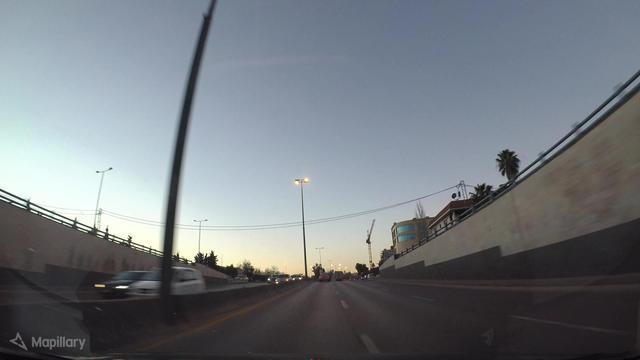
\includegraphics[width=0.31\textwidth,height=0.17\textwidth,keepaspectratio]{qual_msls_day.jpg} &
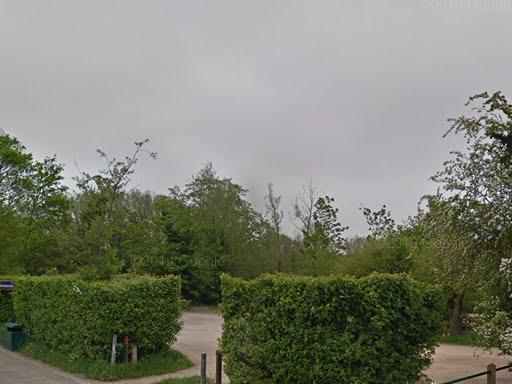
\includegraphics[width=0.31\textwidth,height=0.17\textwidth,keepaspectratio]{qual_svox_day.jpg} &
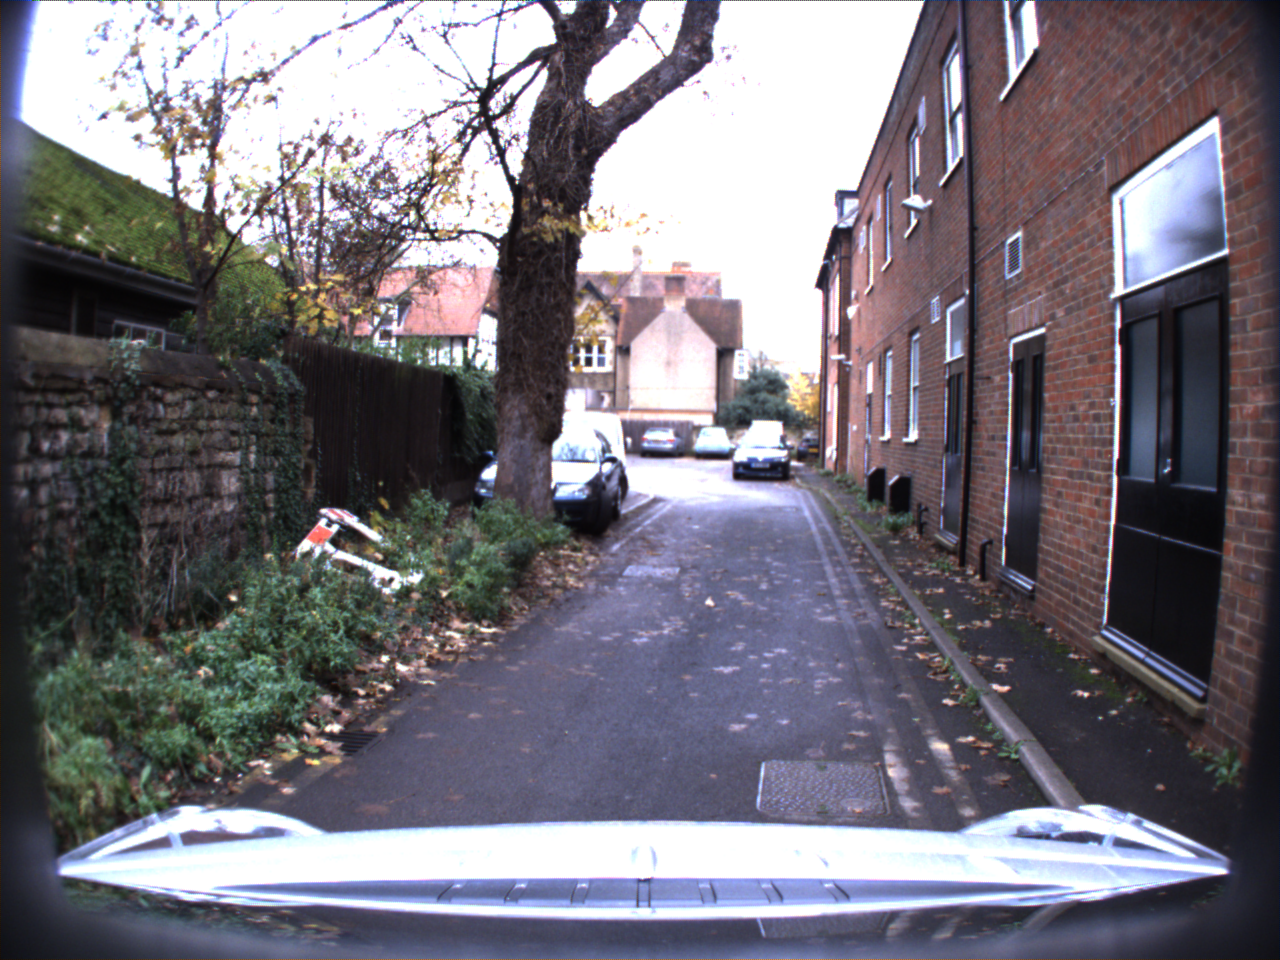
\includegraphics[width=0.31\textwidth,height=0.17\textwidth,keepaspectratio]{qual_robotcar_day.png}\\
\multicolumn{3}{c}{白天源图}\\[2pt]
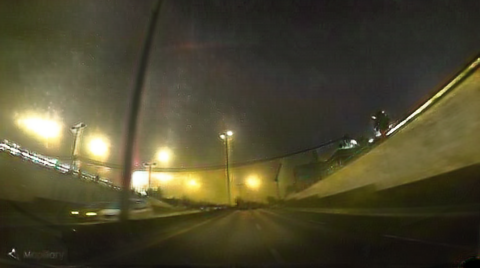
\includegraphics[width=0.31\textwidth,height=0.17\textwidth,keepaspectratio]{qual_msls_fake.png} &
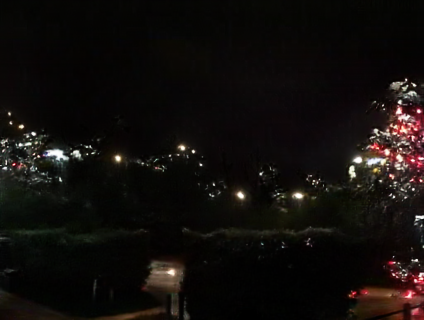
\includegraphics[width=0.31\textwidth,height=0.17\textwidth,keepaspectratio]{qual_svox_fake.png} &
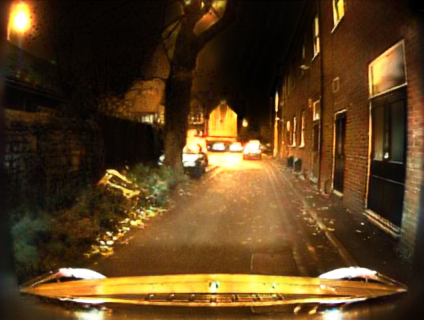
\includegraphics[width=0.31\textwidth,height=0.17\textwidth,keepaspectratio]{qual_robotcar_fake.png}\\
\multicolumn{3}{c}{官方 QS-Attn 目标的 150k 伪夜图}\\[2pt]
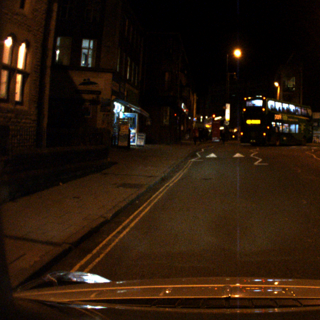
\includegraphics[width=0.31\textwidth,height=0.17\textwidth,keepaspectratio]{qual_real_night_1.png} &
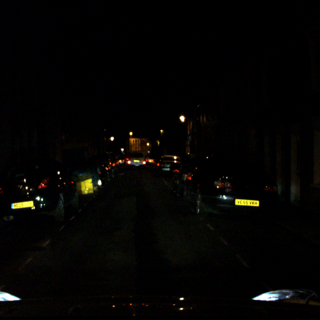
\includegraphics[width=0.31\textwidth,height=0.17\textwidth,keepaspectratio]{qual_real_night_2.png} &
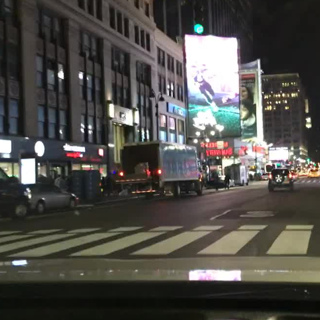
\includegraphics[width=0.31\textwidth,height=0.17\textwidth,keepaspectratio]{qual_real_night_3.png}\\
\multicolumn{3}{c}{真实目标夜域样例（不与上方逐图对应）}
\end{tabular}
\caption{正式生成器定性样例。前两行按列一一对应；第三行为生成训练目标池中的独立真实夜图，用于展示目标域而不是像素配准。}
\label{fig:qualitative-generation}
\end{figure}

\subsection{VPR 监督信号消融}
为分离昼间数据、伪夜数据和教师保持项的影响，四组实验使用完全相同的官方 QS-Attn 150k 伪图、MixVPR 初始化、seed 0 和 optimizer-step 预算。单域主消融使用 compute-matched 配置，避免 day+fake 因每个 source 编码两张图而获得双倍前向计算。计算预算见表~\ref{tab:compute-matching}。各消融目标为
\begin{align}
 \mathcal L_{\mathrm{day}}&=\mathcal L_{\mathrm{LMC}}(z^d,y),\\
 \mathcal L_{\mathrm{fake}}&=\mathcal L_{\mathrm{LMC}}(z^f,y),\\
 \mathcal L_{\mathrm{candidate}}&=\mathcal L_{\mathrm{day+fake}}
 +\frac1B\sum_i\max\left(0,0.95-\cos(z_{s,i}^d,z_{t,i}^d)\right).
\end{align}
其中 $z_s^d$ 和 $z_t^d$ 分别是学生与冻结初始化教师的昼间描述子。保持项先作为候选，其身份只由两个夜间 validation stratum 的预注册规则决定；白天结果只审计代价。该候选最终通过规则，因此等价于式中的正式目标 $\mathcal L_{\mathrm{final}}$。

\begin{table}[htbp]
\centering
\caption{Compute-matched loss 消融预算。编码图像数均为每 epoch。}
\label{tab:compute-matching}
\begin{tabular}{lrrrrr}
\toprule
Loss & source & student 图像 & teacher 图像 & 累积 & optimizer steps\\
\midrule
Day only CM & 120,000 & 120,000 & 0 & 4 & 3,750\tabularnewline
Fake only CM & 120,000 & 120,000 & 0 & 4 & 3,750\tabularnewline
Day + fake & 60,000 & 120,000 & 0 & 2 & 3,750\tabularnewline
Day + fake + preserve & 60,000 & 120,000 & 60,000 & 2 & 3,750\tabularnewline
\bottomrule

\end{tabular}
\end{table}

\subsection{VPR loss 选择}
表~\ref{tab:loss-selection} 是唯一用于决定 preserve/no-preserve 的结果；后续 test 数据集不参与该选择。
\begin{table}[htbp]
\centering
\caption{夜间优先的 loss 选择（R@1，\%）。单侧 $p$ 为 10,000 次分层 paired bootstrap 中非正差值的比例。}
\label{tab:loss-selection}
\resizebox{\textwidth}{!}{%
\begin{tabular}{lrrrrr}
\toprule
Loss & RC-night-val & MSLS-night-val & $S_{\mathrm{night}}$ & 差值 & 单侧 $p$\\
\midrule
day+fake & 90.23 & 60.00 & 75.11 & 0.00 & --\tabularnewline
day+fake+preserve & 90.16 & 65.45 & 77.81 & +2.69 & 0.031\tabularnewline
\bottomrule

\end{tabular}}
\end{table}

表~\ref{tab:loss-suite} 在模型冻结后报告五个夜间/过渡条件。它只分析域泛化，不能用于重新选择 loss；最后一列只平均 RobotCar、SVOX-night 与 Tokyo-night 三个独立夜间 test，不包含 MSLS validation 或 Tokyo sunset。
\begin{table}[htbp]
\centering
\caption{四种 VPR loss 的冻结 R@1（\%）。MSLS 为 validation，Tokyo-S 为 transition。}
\label{tab:loss-suite}
\resizebox{\textwidth}{!}{%
\begin{tabular}{lrrrrrr}
\toprule
Loss & RC-10m/$30^\circ$ & SVOX-N & MSLS-N val & Tokyo-N & Tokyo-S & 夜间 test 宏平均\\
\midrule
Day only CM & 67.78 & 40.22 & 36.36 & 54.61 & 75.89 & 54.20\tabularnewline
Fake only CM & 77.59 & 57.72 & 45.45 & 59.57 & 76.60 & 64.96\tabularnewline
Day + fake & 88.41 & 76.31 & 60.00 & 62.41 & 75.18 & 75.71\tabularnewline
Day + fake + preserve & 88.24 & 76.06 & 65.45 & 60.99 & 75.89 & 75.10\tabularnewline
\bottomrule

\end{tabular}}
\end{table}

无 preserve 与 preserve 的 $S_{\mathrm{night}}$ 分别为 75.11\% 和 77.81\%，提升 2.69 个百分点。10,000 次分层重采样中正差值比例为 96.94\%，非正比例与单侧经验 $p$ 值均为 0.0306，满足小于 5\% 的选择条件。双侧 percentile 95\% CI 约为 $[-0.04,6.26]$ 个百分点，数值下界接近 0；这反映 MSLS-night 仅有 55 个有效 query 的不确定性。RobotCar night val 单项下降 0.071 个百分点，但 MSLS night 提升 5.45 个百分点，因此等权夜间宏平均仍改善。preserve 的保留不依赖白天或 test 结果。

旧单域实验只匹配 source 数量，没有匹配图像前向量，其数值不用于主消融结论。compute-matched 训练显示 day-only 和 fake-only 的 RobotCar val best R@1 分别为 69.76\% 与 80.03\%，其 best epoch 分别为 4 与 13。Tokyo-sunset 单列为昼夜过渡条件，伪夜适配在该条件上不保证单调改善。

\subsection{白天能力保持}
\begin{table}[htbp]
\centering
\caption{冻结后的白天测试 R@1（\%）。MSLS-day-val 与 SVOX-day-val 只用于前述选择，不列入本表。}
\label{tab:day-ability}
\begin{tabular}{lrrrrr}
\toprule
模型/Loss & RC-day & SVOX-day & SVOX-sun & Tokyo-day & 宏平均\\
\midrule
MixVPR official & 98.35 & 96.69 & 79.16 & 84.40 & 89.65\tabularnewline
Day only CM & 98.68 & 96.29 & 83.37 & 84.40 & 90.69\tabularnewline
Fake only CM & 98.68 & 96.32 & 79.86 & 84.40 & 89.81\tabularnewline
Day + fake & 98.29 & 95.75 & 82.55 & 80.85 & 89.36\tabularnewline
Day + fake + preserve & 98.35 & 95.81 & 82.55 & 80.14 & 89.21\tabularnewline
\bottomrule

\end{tabular}
\end{table}

白天冻结测试给出重要的安全性边界。官方初始化、day-only CM、fake-only CM、day+fake 和 preserve 的四项宏平均分别为 89.65\%、90.69\%、89.81\%、89.36\% 和 89.21\%。preserve 相对无 preserve 在 MSLS-day-val 与 SVOX-day-val 上分别提高约 0.39 和 0.18 个百分点，但在完全冻结的四项 day test 上低 0.15 个百分点，并比官方初始化低 0.44 个百分点。它在 SVOX-sun 上比初始化高 3.39 个百分点，却在 Tokyo-day 上低 4.26 个百分点。因此 preserve 是夜间收益优先、白天变化受审计的训练锚点，而不是“保证白天 Recall 更高”的模块。

\subsection{统一 R@1 主表}
表~\ref{tab:main-r1} 区分三种实验身份：A2B-LightVPR 与 NetVLAD 使用官方 QS-Attn 150k 伪图完成昼/伪夜适配；CosPlace、EigenPlaces、MixVPR 和 DINOv2 行为固定官方权重的零样本结果；NocPlace 行为自有数据上的协议复现。所有行共享查询协议；各模型原生预处理结果属于系统比较，严格适配增益另要求完整评测指纹一致。
\begin{table}[htbp]
\centering
\caption{统一协议 R@1（\%）。MSLS-N 是 validation，Tokyo-S 是 transition；宏平均只含三个独立夜间 test。}
\label{tab:main-r1}
\resizebox{\textwidth}{!}{%
\begin{tabular}{lrrrrrr}
\toprule
模型 & RC-10m/$30^\circ$ & SVOX-N & MSLS-N val & Tokyo-N & Tokyo-S & 夜间 test 宏平均\\
\midrule
A2B-LightVPR, seed 0（day+fake+preserve） & 88.24 & 76.06 & 65.45 & 60.99 & 75.89 & 75.10\tabularnewline
NetVLAD-4096（官方 QS 伪图适配） & 67.61 & 38.27 & 14.55 & 39.72 & 68.09 & 48.54\tabularnewline
MixVPR-R50-512（官方零样本） & 65.94 & 47.27 & 34.55 & 51.77 & 74.47 & 54.99\tabularnewline
MixVPR-R50-4096（官方零样本） & 75.59 & 63.30 & 43.64 & 62.41 & 82.98 & 67.10\tabularnewline
CosPlace-R50-512（官方零样本） & 47.05 & 46.66 & 23.64 & 51.77 & 74.47 & 48.49\tabularnewline
EigenPlaces-R50-512（官方零样本） & 54.46 & 46.05 & 16.36 & 51.77 & 78.01 & 50.76\tabularnewline
EigenPlaces-R50-2048（官方零样本） & 56.24 & 50.06 & 21.82 & 53.19 & 80.14 & 53.17\tabularnewline
SALAD-DINOv2-544（官方零样本） & 92.08 & 92.47 & 96.36 & 80.14 & 82.27 & 88.23\tabularnewline
CricaVPR-DINOv2-10752（官方零样本） & 89.35 & 85.30 & 70.91 & 73.76 & 83.69 & 82.80\tabularnewline
BoQ-DINOv2-12288（官方零样本） & 96.88 & 97.69 & 100.00 & 87.23 & 88.65 & 93.93\tabularnewline
NocPlace OD=true（协议复现） & 63.88 & 38.76 & 47.27 & 46.81 & 60.28 & 49.82\tabularnewline
NocPlace OD=false（协议复现） & 70.35 & 54.31 & 38.18 & 54.61 & 65.96 & 59.76\tabularnewline
\bottomrule

\end{tabular}}
\end{table}

最终 seed 0 A2B-LightVPR 在 RobotCar、SVOX-night 与 Tokyo-night 上分别达到 88.24\%、76.06\% 和 60.99\%，独立夜间 test 宏平均为 75.10\%。MSLS-night 的 65.45\% 属于参与 loss 选择的 validation，Tokyo-sunset 的 75.89\% 属于过渡条件，二者均不混入该宏平均。相对无 preserve，最终模型主要收益出现在 MSLS validation，而部分冻结 test 有轻微波动；这说明 preserve 是按预注册夜间验证规则选择，并非观察 test 后追求逐项占优。BoQ 与 SALAD 的绝对 Recall 更高，因此本文优势是紧凑描述子与跨域精度的折中，而非精度上界。

\subsection{官方 QS-Attn 伪夜适配增益}
为避免将最终结果误归因于 MixVPR 本身，表~\ref{tab:adaptation-gain} 只在官方初始化与最终 checkpoint 的 \texttt{evaluation\_fingerprint} 完全一致时计算适配增益。当前原生官方 MixVPR 使用直接缩放，而 A2B 使用 $320\times320$ fit-and-pad；原生结果保留在系统主表，但不能用于该受控增益表。待统一 fit-and-pad 基线完成前，对应单元保持 ``--''。
\begin{table}[htbp]
\centering
\caption{最终 day+fake+preserve 模型相对官方零样本 MixVPR-R50-512 的 R@1 增益（百分点）。}
\label{tab:adaptation-gain}
\begin{tabular}{lrrr}
\toprule
协议 & 官方零样本 & A2B-LightVPR & 差值\\
\midrule
RC-10m/30$^\circ$ & 64.49 & 88.24 & +23.75\tabularnewline
SVOX-N & 43.26 & 76.06 & +32.81\tabularnewline
MSLS-N (val) & 32.73 & 65.45 & +32.73\tabularnewline
Tokyo-N & 52.48 & 60.99 & +8.51\tabularnewline
Tokyo-S (transition) & 73.76 & 75.89 & +2.13\tabularnewline
\bottomrule

\end{tabular}
\end{table}

这一约束修正了早期版本把不同 resize 结果直接相减的问题。正式增益数值必须由 $320\times320$ fit-and-pad 的官方 MixVPR 重新提取，并在表格导出时通过完整评测指纹检查；脚本拒绝用原生 direct-resize 数值自动补位。

\begin{table}[htbp]
\centering
\caption{统一 $320\times320$ fit-and-pad 的受控 R@1（\%）。MSLS-N 是 validation，Tokyo-S 是 transition。}
\label{tab:controlled-preprocessing}
\resizebox{\textwidth}{!}{%
\begin{tabular}{lrrrrrr}
\toprule
模型 & RC-10m/$30^\circ$ & SVOX-N & MSLS-N val & Tokyo-N & Tokyo-S & 夜间 test 宏平均\\
\midrule
A2B-LightVPR & 88.24 & 76.06 & 65.45 & 60.99 & 75.89 & 75.10\tabularnewline
MixVPR official & 64.49 & 43.26 & 32.73 & 52.48 & 73.76 & 53.41\tabularnewline
NocPlace OD=true & 35.56 & 19.32 & 45.45 & 38.30 & 56.03 & 31.06\tabularnewline
NocPlace OD=false & 41.25 & 25.39 & 29.09 & 46.81 & 61.70 & 37.82\tabularnewline
\bottomrule

\end{tabular}}
\end{table}

表~\ref{tab:controlled-preprocessing} 与主表的角色不同：前者固定输入变换，分离训练方法差异；后者保留各参考模型官方原生预处理，表示完整系统表现。两种结果不得在同一“适配增益”列中混算。

NetVLAD 适配后在 RobotCar、SVOX、MSLS validation、Tokyo-night 与 Tokyo-sunset 上的 R@1 分别为 67.61\%、38.27\%、14.55\%、39.72\% 和 68.09\%。其 RobotCar validation 曾达到 71.90\%，但跨数据集结果明显低于最终 MixVPR，尤其 MSLS 仅为 14.55\%。这说明相同伪夜适配可以改善经典聚合器，却不能消除架构与初始化本身的泛化差异；NetVLAD 更适合作为经典基线，而不是本文部署候选。

\subsection{相对 NocPlace 的逐查询统计}
表~\ref{tab:nocplace-bootstrap} 使用最终 day+fake+preserve checkpoint 计算。OD=true 表示原始 CosPlace 编码白天 database、适配模型编码夜间 query；OD=false 表示适配模型编码两侧。逐查询 bootstrap 要求查询协议指纹一致；只有统一 $320\times320$ fit-and-pad 后的补充比较才属于同预处理受控结果。
\begin{table}[htbp]
\centering
\caption{最终 A2B-LightVPR 相对本地 NocPlace 的 R@1 paired bootstrap（\%，10,000 次）。}
\label{tab:nocplace-bootstrap}
\begin{tabular}{llrrrr}
\toprule
NocPlace & 协议 & A2B & NocPlace & 差值 & 95\% CI\\
\midrule
OD=true & RC-10m/30$^\circ$ & 88.24 & 63.88 & 24.10 & [21.79, 26.53]\tabularnewline
OD=true & SVOX-N & 76.06 & 38.76 & 37.30 & [33.29, 41.19]\tabularnewline
OD=true & MSLS-N (val) & 65.45 & 47.27 & 18.18 & [3.64, 32.73]\tabularnewline
OD=true & Tokyo-N & 60.99 & 46.81 & 5.33 & [1.87, 8.80]\tabularnewline
OD=true & Tokyo-S (transition) & 75.89 & 60.28 & 5.87 & [2.93, 9.07]\tabularnewline
OD=false & RC-10m/30$^\circ$ & 88.24 & 70.35 & 17.71 & [15.50, 19.91]\tabularnewline
OD=false & SVOX-N & 76.06 & 54.31 & 21.75 & [18.10, 25.52]\tabularnewline
OD=false & MSLS-N (val) & 65.45 & 38.18 & 27.27 & [12.73, 41.82]\tabularnewline
OD=false & Tokyo-N & 60.99 & 54.61 & 2.40 & [-0.80, 5.60]\tabularnewline
OD=false & Tokyo-S (transition) & 75.89 & 65.96 & 3.73 & [0.53, 6.93]\tabularnewline
\bottomrule

\end{tabular}
\end{table}

现有 NocPlace 原生系统结果说明 A2B 在多个夜间数据集上具有更高点估计，但两者输入预处理不同，不能把差值解释为纯训练方法增益。统一 fit-and-pad 补测完成后，正文将同时保留“同输入受控比较”和“各模型原生系统比较”，并分别报告点估计与置信区间。

\subsection{DINOv2 精度上界}
SALAD、CricaVPR 和 BoQ 均使用官方固定 checkpoint。BoQ 在 MSLS 的 55 个有效查询上达到 100\% R@1，但该数据集样本较少，应结合 R@5/R@10、MRR 和置信区间解释。CricaVPR 在 MSLS 与 SVOX 上低于 SALAD，说明更长描述子并不自动保证每个数据集更强。所有 DINOv2 模型的完整指标见附录表~\ref{tab:appendix-metrics}。

\subsection{资源比较}
\begin{table}[htbp]
\centering
\caption{同设备 PyTorch FP16 batch-1 资源对照。百万图内存按 FP32 描述子计算。}
\label{tab:resources}
\resizebox{\textwidth}{!}{%
\begin{tabular}{lrrrrrrr}
\toprule
模型 & 参数/M & CKPT/MiB & 维度 & 百万图/GiB & 峰值/MiB & p50/ms & p95/ms\\
\midrule
mixvpr-r50-512 & 10.09 & 38.7 & 512 & 1.91 & 73.5 & 3.22 & 3.53\tabularnewline
mixvpr-r50-4096 & 10.88 & 41.7 & 4096 & 15.26 & 76.4 & 3.23 & 3.62\tabularnewline
cosplace-r50-512 & 24.56 & 94.0 & 512 & 1.91 & 155.0 & 3.56 & 3.69\tabularnewline
eigenplaces-r50-512 & 24.56 & 94.0 & 512 & 1.91 & 155.6 & 3.54 & 3.69\tabularnewline
eigenplaces-r50-2048 & 27.70 & 106.0 & 2048 & 7.63 & 174.2 & 3.56 & 3.65\tabularnewline
salad-dinov2-544 & 87.80 & 335.0 & 544 & 2.03 & 363.1 & 14.25 & 14.58\tabularnewline
cricavpr-dinov2-b-10752 & 106.76 & 561.6 & 10752 & 40.05 & 710.0 & 15.89 & 16.21\tabularnewline
boq-dinov2-12288 & 95.21 & 363.3 & 12288 & 45.78 & 396.5 & 12.35 & 12.60\tabularnewline
netvlad-vgg16-pitts4096 & 149.00 & 1080.4 & 4096 & 15.26 & 860.4 & 10.83 & 11.36\tabularnewline
\bottomrule

\end{tabular}}
\end{table}

MixVPR-R50-512 为 10.09M 参数、512 维，p95 为 3.53 ms，百万图 FP32 描述子为 1.91 GiB。相对 SALAD，其描述子存储只减少约 5.9\%，主要优势来自更少参数、更低峰值显存和约 4.13 倍单图速度。相对 CricaVPR 与 BoQ，描述子存储分别减少约 95.24\% 与 95.83\%，速度分别约为 4.59 倍与 3.57 倍。该比较只描述当前软硬件协议下的相对关系。

\section{讨论}
\subsection{同一编码器为何能处理两个域}
共享编码器并不是要求白天和夜间像素或描述子完全一致。地点分类器为每个地点学习一个决策方向，同地点的 day/fake 可以位于该方向附近的不同区域。多地点、多城市和两域样本共同训练后，稳定的道路边界、建筑轮廓和视角布局更容易成为分类依据，而不稳定的亮度和颜色贡献会降低。生成图提供的价值是让模型在保留地点标签的情况下看到夜间外观扰动。

这也解释了为什么逐图强行把 day 与 fake 描述子拉到同一点未必合理：域差异可能包含曝光可靠性、局部遮挡和动态光源等真实变化。本文的 preserve 不直接对齐 day/fake，而是以冻结初始化教师为白天表征设置锚点。双夜间 stratum 选择说明该约束提高了夜间 validation 宏平均；冻结 day test 又说明白天总体变化虽小，但并非所有数据集都提升。两者共同限定了保持项的合理结论范围。

\subsection{为何需要两个夜间 validation stratum}
只用 RobotCar validation 选择 loss 容易偏向单一城市、固定路线和特定相机。MSLS night validation 只有 55 个有效 query，却提供跨城市和不同采集设备的独立信号。等权宏平均避免 RobotCar 查询数量支配结果，分层 bootstrap 保留各自查询结构。该规则允许单个 stratum 轻微下降，只要求夜间宏平均为正且单侧非正概率低于 5\%；本实验中 RobotCar night 的 $-0.071$ 个百分点正是这一情形。由于 MSLS night 样本很少，本文同时给出双侧 CI，不把 5.45 个百分点点估计视为精确总体效应。白天验证与测试回答的是“夜间收益付出了多少白天代价”，而不是“是否选择 preserve”。

\subsection{生成指标与 Recall 的边界}
FID 和 KID 衡量生成图与真实夜图的特征分布，L2、PSNR 和 SSIM 衡量像素或局部结构；它们都不观察地理正样本集合和检索排名。本实验中 50k checkpoint 的 FID/KID 最优，而所有 VPR 训练预先固定使用 150k checkpoint。因此本文不使用 FID 替代下游选择，也不将更低的生成指标直接解释为更高的 VPR Recall。

\subsection{结论边界}
NightCities 与 SF-XL-NC 不公开，因此本地 NocPlace 结果不能替代论文原始表格。Tokyo 与 RobotCar 也使用本项目 split 和输入协议。本文证明的是：在可审计的自有数据上，官方 QS-Attn 离线昼夜生成与双域地点监督能够改善紧凑 VPR；本文不声称复现 NocPlace 的原始数据，也不声称提出新的生成器或 VPR backbone。

正文主结果是预先固定的 seed 0，而非从多个随机种子中挑选的最好值。逐查询 bootstrap 只表示给定 checkpoint 与给定测试查询下的抽样不确定性，不表示训练随机性，因而不能据此声称多 seed 稳定性。已有 seed 1/2 仅在附录作描述性补充，且没有对应的 no-preserve 多 seed 对照。MSLS night 仅有 55 个有效 query，其点估计对少数查询较敏感，因此本文使用分层置信区间而不单独依赖该行的 R@1。

\section{结论}
本文将官方 QS-Attn 昼夜翻译作为离线数据构建步骤，并以双域地点监督和训练期白天保持项适配单一 MixVPR-R50-512 编码器。preserve 按预注册的双夜间验证规则被选中，使 $S_{\mathrm{night}}$ 提高 2.69 个百分点，单侧 bootstrap $p=0.031$。最终 seed 0 在 RobotCar 10 m/$30^\circ$、SVOX-night 和 Tokyo-night 上的 R@1 分别为 88.24\%、76.06\% 和 60.99\%，独立夜间 test 宏平均为 75.10\%。冻结白天 test 宏平均相对无 preserve 仅低 0.15 个百分点、相对初始化低 0.44 个百分点，说明系统获得的是明显夜间收益下的小幅白天能力折中，而不是无代价的全域提升。DINOv2 强模型仍提供更高的绝对精度；本文 512 维候选的价值在于更少参数、更短描述子、更低显存和更快推理。

\appendix
\section{全部 VPR 模型的完整检索指标}
\begingroup
\scriptsize
\setlength{\tabcolsep}{3pt}
\begin{longtable}{llrrrrrrr}
\caption{逐数据集 R@1/R@5/R@10/MRR（\%）及样本数。}\label{tab:appendix-metrics}\\
\toprule
模型 & 数据集 & R@1 & R@5 & R@10 & MRR & DB & Query & 有效 Query\\
\midrule
\endfirsthead
\toprule
模型 & 数据集 & R@1 & R@5 & R@10 & MRR & DB & Query & 有效 Query\\
\midrule
\endhead
A2B-LightVPR & RC-10m/30$^\circ$ & 88.24 & 95.32 & 97.16 & 91.32 & 1810 & 1813 & 1794\tabularnewline
A2B-LightVPR & SVOX-N & 76.06 & 86.76 & 89.79 & 80.64 & 17166 & 823 & 823\tabularnewline
A2B-LightVPR & MSLS-N (val) & 65.45 & 80.00 & 85.45 & 71.48 & 18886 & 55 & 55\tabularnewline
A2B-LightVPR & Tokyo-N & 60.99 & 75.18 & 81.56 & 67.50 & 75984 & 375 & 141\tabularnewline
A2B-LightVPR & Tokyo-S (transition) & 75.89 & 83.69 & 86.52 & 79.69 & 75984 & 375 & 141\tabularnewline
NetVLAD-adapted & RC-10m/30$^\circ$ & 67.61 & 83.72 & 89.30 & 74.73 & 1810 & 1813 & 1794\tabularnewline
NetVLAD-adapted & SVOX-N & 38.27 & 58.81 & 64.88 & 46.96 & 17166 & 823 & 823\tabularnewline
NetVLAD-adapted & MSLS-N (val) & 14.55 & 29.09 & 34.55 & 21.62 & 18886 & 55 & 55\tabularnewline
NetVLAD-adapted & Tokyo-N & 39.72 & 52.48 & 63.12 & 45.36 & 75984 & 375 & 141\tabularnewline
NetVLAD-adapted & Tokyo-S (transition) & 68.09 & 82.27 & 84.40 & 74.10 & 75984 & 375 & 141\tabularnewline
MixVPR-512 & RC-10m/30$^\circ$ & 65.94 & 83.56 & 89.02 & 73.45 & 1810 & 1813 & 1794\tabularnewline
MixVPR-512 & SVOX-N & 47.27 & 63.91 & 72.05 & 54.49 & 17166 & 823 & 823\tabularnewline
MixVPR-512 & MSLS-N (val) & 34.55 & 50.91 & 60.00 & 41.63 & 18886 & 55 & 55\tabularnewline
MixVPR-512 & Tokyo-N & 51.77 & 65.25 & 73.76 & 57.21 & 75984 & 375 & 141\tabularnewline
MixVPR-512 & Tokyo-S (transition) & 74.47 & 85.82 & 88.65 & 79.23 & 75984 & 375 & 141\tabularnewline
MixVPR-4096 & RC-10m/30$^\circ$ & 75.59 & 90.69 & 93.98 & 81.97 & 1810 & 1813 & 1794\tabularnewline
MixVPR-4096 & SVOX-N & 63.30 & 78.74 & 82.99 & 69.98 & 17166 & 823 & 823\tabularnewline
MixVPR-4096 & MSLS-N (val) & 43.64 & 70.91 & 72.73 & 55.93 & 18886 & 55 & 55\tabularnewline
MixVPR-4096 & Tokyo-N & 62.41 & 78.72 & 81.56 & 69.28 & 75984 & 375 & 141\tabularnewline
MixVPR-4096 & Tokyo-S (transition) & 82.98 & 89.36 & 90.07 & 85.76 & 75984 & 375 & 141\tabularnewline
CosPlace-512 & RC-10m/30$^\circ$ & 47.05 & 61.04 & 68.56 & 53.19 & 1810 & 1813 & 1794\tabularnewline
CosPlace-512 & SVOX-N & 46.66 & 65.37 & 72.78 & 53.92 & 17166 & 823 & 823\tabularnewline
CosPlace-512 & MSLS-N (val) & 23.64 & 34.55 & 43.64 & 29.12 & 18886 & 55 & 55\tabularnewline
CosPlace-512 & Tokyo-N & 51.77 & 65.25 & 69.50 & 57.14 & 75984 & 375 & 141\tabularnewline
CosPlace-512 & Tokyo-S (transition) & 74.47 & 84.40 & 87.94 & 79.04 & 75984 & 375 & 141\tabularnewline
EigenPlaces-512 & RC-10m/30$^\circ$ & 54.46 & 72.13 & 78.87 & 62.02 & 1810 & 1813 & 1794\tabularnewline
EigenPlaces-512 & SVOX-N & 46.05 & 67.68 & 75.70 & 55.11 & 17166 & 823 & 823\tabularnewline
EigenPlaces-512 & MSLS-N (val) & 16.36 & 23.64 & 25.45 & 19.88 & 18886 & 55 & 55\tabularnewline
EigenPlaces-512 & Tokyo-N & 51.77 & 66.67 & 71.63 & 57.91 & 75984 & 375 & 141\tabularnewline
EigenPlaces-512 & Tokyo-S (transition) & 78.01 & 85.11 & 88.65 & 81.10 & 75984 & 375 & 141\tabularnewline
EigenPlaces-2048 & RC-10m/30$^\circ$ & 56.24 & 72.46 & 78.21 & 62.99 & 1810 & 1813 & 1794\tabularnewline
EigenPlaces-2048 & SVOX-N & 50.06 & 70.35 & 76.79 & 58.60 & 17166 & 823 & 823\tabularnewline
EigenPlaces-2048 & MSLS-N (val) & 21.82 & 29.09 & 38.18 & 25.24 & 18886 & 55 & 55\tabularnewline
EigenPlaces-2048 & Tokyo-N & 53.19 & 70.21 & 77.30 & 59.80 & 75984 & 375 & 141\tabularnewline
EigenPlaces-2048 & Tokyo-S (transition) & 80.14 & 86.52 & 90.07 & 83.13 & 75984 & 375 & 141\tabularnewline
SALAD & RC-10m/30$^\circ$ & 92.08 & 99.00 & 99.67 & 95.15 & 1810 & 1813 & 1794\tabularnewline
SALAD & SVOX-N & 92.47 & 97.45 & 98.91 & 94.59 & 17166 & 823 & 823\tabularnewline
SALAD & MSLS-N (val) & 96.36 & 100.00 & 100.00 & 97.88 & 18886 & 55 & 55\tabularnewline
SALAD & Tokyo-N & 80.14 & 87.94 & 90.07 & 83.50 & 75984 & 375 & 141\tabularnewline
SALAD & Tokyo-S (transition) & 82.27 & 90.78 & 92.20 & 85.45 & 75984 & 375 & 141\tabularnewline
CricaVPR & RC-10m/30$^\circ$ & 89.35 & 96.82 & 98.33 & 92.56 & 1810 & 1813 & 1794\tabularnewline
CricaVPR & SVOX-N & 85.30 & 93.92 & 96.84 & 88.96 & 17166 & 823 & 823\tabularnewline
CricaVPR & MSLS-N (val) & 70.91 & 85.45 & 87.27 & 76.52 & 18886 & 55 & 55\tabularnewline
CricaVPR & Tokyo-N & 73.76 & 87.23 & 88.65 & 79.90 & 75984 & 375 & 141\tabularnewline
CricaVPR & Tokyo-S (transition) & 83.69 & 93.62 & 94.33 & 87.87 & 75984 & 375 & 141\tabularnewline
BoQ & RC-10m/30$^\circ$ & 96.88 & 99.94 & 100.00 & 98.21 & 1810 & 1813 & 1794\tabularnewline
BoQ & SVOX-N & 97.69 & 99.51 & 99.76 & 98.54 & 17166 & 823 & 823\tabularnewline
BoQ & MSLS-N (val) & 100.00 & 100.00 & 100.00 & 100.00 & 18886 & 55 & 55\tabularnewline
BoQ & Tokyo-N & 87.23 & 93.62 & 94.33 & 89.52 & 75984 & 375 & 141\tabularnewline
BoQ & Tokyo-S (transition) & 88.65 & 95.04 & 96.45 & 90.91 & 75984 & 375 & 141\tabularnewline
NocPlace-OD-true & RC-10m/30$^\circ$ & 63.88 & 81.33 & 86.29 & 71.33 & 1810 & 1813 & 1794\tabularnewline
NocPlace-OD-true & SVOX-N & 38.76 & 57.84 & 65.74 & 46.54 & 17166 & 823 & 823\tabularnewline
NocPlace-OD-true & MSLS-N (val) & 47.27 & 54.55 & 61.82 & 51.27 & 18886 & 55 & 55\tabularnewline
NocPlace-OD-true & Tokyo-N & 46.81 & 63.83 & 70.92 & 53.85 & 75984 & 375 & 141\tabularnewline
NocPlace-OD-true & Tokyo-S (transition) & 60.28 & 71.63 & 75.89 & 65.62 & 75984 & 375 & 141\tabularnewline
NocPlace-OD-false & RC-10m/30$^\circ$ & 70.35 & 83.95 & 88.29 & 75.94 & 1810 & 1813 & 1794\tabularnewline
NocPlace-OD-false & SVOX-N & 54.31 & 71.32 & 77.52 & 61.57 & 17166 & 823 & 823\tabularnewline
NocPlace-OD-false & MSLS-N (val) & 38.18 & 60.00 & 69.09 & 47.49 & 18886 & 55 & 55\tabularnewline
NocPlace-OD-false & Tokyo-N & 54.61 & 68.79 & 75.18 & 60.30 & 75984 & 375 & 141\tabularnewline
NocPlace-OD-false & Tokyo-S (transition) & 65.96 & 78.72 & 80.14 & 70.87 & 75984 & 375 & 141\tabularnewline
\bottomrule

\end{longtable}
\endgroup

\section{Protocol fingerprints}
\begin{longtable}{p{4.2cm}p{5.5cm}p{5.5cm}}
\caption{查询协议与完整评测指纹。查询指纹控制正样本和逐查询配对；评测指纹进一步控制预处理。}\\
\toprule
模型/协议 & Query protocol SHA256 & Evaluation SHA256\\
\midrule
\endfirsthead
\toprule
模型/协议 & Query protocol SHA256 & Evaluation SHA256\\
\midrule
\endhead
A2B-LightVPR / RC-10m/30$^\circ$ & \texttt{\seqsplit{5cd4a6434b19289caceb6f0f3f587f2baf5900ebd3bd3daab7e35ca38d81be6a}} & \texttt{\seqsplit{548464995f12727476f6cf2831ef13b93c7bf600a5f2673e82880066c4a9188f}}\tabularnewline
A2B-LightVPR / SVOX-N & \texttt{\seqsplit{2986d465c078b67bd421e441292cd6d8d8bd50cb51e0dae867b230d8fb646190}} & \texttt{\seqsplit{edf532fcc1caee318c8bf20d8d0c84efc9e4751d28d55619491a01b1853ebd87}}\tabularnewline
A2B-LightVPR / MSLS-N (val) & \texttt{\seqsplit{ba41a88f4710c0a17aa7a854d0d97a59ee10c3e91c377b47a7b989bfdce726df}} & \texttt{\seqsplit{d64fe11e31a8fc25432322df8794bc3cef2ade22473927951c1e96f72137f29d}}\tabularnewline
A2B-LightVPR / Tokyo-N & \texttt{\seqsplit{82169b63f768c1c616c518cdc3d3f3b07a781ff93c2fef2d865db0e20cd462f2}} & \texttt{\seqsplit{39d54681a7e645cfffcfb91a3a735b749a061e36f82092627ef41a1c819153f0}}\tabularnewline
A2B-LightVPR / Tokyo-S (transition) & \texttt{\seqsplit{5b2085e3091f02c57be9acf1b46ff439fd167e51258ab8cab342b9552bd57168}} & \texttt{\seqsplit{4e4be67cf4455a838fb455f2fd1f953489e573b23b67345ac0dabde68da7b473}}\tabularnewline
NetVLAD-adapted / RC-10m/30$^\circ$ & \texttt{\seqsplit{5cd4a6434b19289caceb6f0f3f587f2baf5900ebd3bd3daab7e35ca38d81be6a}} & \texttt{\seqsplit{legacy/pending}}\tabularnewline
NetVLAD-adapted / SVOX-N & \texttt{\seqsplit{2986d465c078b67bd421e441292cd6d8d8bd50cb51e0dae867b230d8fb646190}} & \texttt{\seqsplit{legacy/pending}}\tabularnewline
NetVLAD-adapted / MSLS-N (val) & \texttt{\seqsplit{ba41a88f4710c0a17aa7a854d0d97a59ee10c3e91c377b47a7b989bfdce726df}} & \texttt{\seqsplit{legacy/pending}}\tabularnewline
NetVLAD-adapted / Tokyo-N & \texttt{\seqsplit{82169b63f768c1c616c518cdc3d3f3b07a781ff93c2fef2d865db0e20cd462f2}} & \texttt{\seqsplit{legacy/pending}}\tabularnewline
NetVLAD-adapted / Tokyo-S (transition) & \texttt{\seqsplit{5b2085e3091f02c57be9acf1b46ff439fd167e51258ab8cab342b9552bd57168}} & \texttt{\seqsplit{legacy/pending}}\tabularnewline
MixVPR-512 / RC-10m/30$^\circ$ & \texttt{\seqsplit{5cd4a6434b19289caceb6f0f3f587f2baf5900ebd3bd3daab7e35ca38d81be6a}} & \texttt{\seqsplit{legacy/pending}}\tabularnewline
MixVPR-512 / SVOX-N & \texttt{\seqsplit{2986d465c078b67bd421e441292cd6d8d8bd50cb51e0dae867b230d8fb646190}} & \texttt{\seqsplit{legacy/pending}}\tabularnewline
MixVPR-512 / MSLS-N (val) & \texttt{\seqsplit{ba41a88f4710c0a17aa7a854d0d97a59ee10c3e91c377b47a7b989bfdce726df}} & \texttt{\seqsplit{legacy/pending}}\tabularnewline
MixVPR-512 / Tokyo-N & \texttt{\seqsplit{82169b63f768c1c616c518cdc3d3f3b07a781ff93c2fef2d865db0e20cd462f2}} & \texttt{\seqsplit{legacy/pending}}\tabularnewline
MixVPR-512 / Tokyo-S (transition) & \texttt{\seqsplit{5b2085e3091f02c57be9acf1b46ff439fd167e51258ab8cab342b9552bd57168}} & \texttt{\seqsplit{legacy/pending}}\tabularnewline
MixVPR-4096 / RC-10m/30$^\circ$ & \texttt{\seqsplit{5cd4a6434b19289caceb6f0f3f587f2baf5900ebd3bd3daab7e35ca38d81be6a}} & \texttt{\seqsplit{legacy/pending}}\tabularnewline
MixVPR-4096 / SVOX-N & \texttt{\seqsplit{2986d465c078b67bd421e441292cd6d8d8bd50cb51e0dae867b230d8fb646190}} & \texttt{\seqsplit{legacy/pending}}\tabularnewline
MixVPR-4096 / MSLS-N (val) & \texttt{\seqsplit{ba41a88f4710c0a17aa7a854d0d97a59ee10c3e91c377b47a7b989bfdce726df}} & \texttt{\seqsplit{legacy/pending}}\tabularnewline
MixVPR-4096 / Tokyo-N & \texttt{\seqsplit{82169b63f768c1c616c518cdc3d3f3b07a781ff93c2fef2d865db0e20cd462f2}} & \texttt{\seqsplit{legacy/pending}}\tabularnewline
MixVPR-4096 / Tokyo-S (transition) & \texttt{\seqsplit{5b2085e3091f02c57be9acf1b46ff439fd167e51258ab8cab342b9552bd57168}} & \texttt{\seqsplit{legacy/pending}}\tabularnewline
CosPlace-512 / RC-10m/30$^\circ$ & \texttt{\seqsplit{5cd4a6434b19289caceb6f0f3f587f2baf5900ebd3bd3daab7e35ca38d81be6a}} & \texttt{\seqsplit{legacy/pending}}\tabularnewline
CosPlace-512 / SVOX-N & \texttt{\seqsplit{2986d465c078b67bd421e441292cd6d8d8bd50cb51e0dae867b230d8fb646190}} & \texttt{\seqsplit{legacy/pending}}\tabularnewline
CosPlace-512 / MSLS-N (val) & \texttt{\seqsplit{ba41a88f4710c0a17aa7a854d0d97a59ee10c3e91c377b47a7b989bfdce726df}} & \texttt{\seqsplit{legacy/pending}}\tabularnewline
CosPlace-512 / Tokyo-N & \texttt{\seqsplit{82169b63f768c1c616c518cdc3d3f3b07a781ff93c2fef2d865db0e20cd462f2}} & \texttt{\seqsplit{legacy/pending}}\tabularnewline
CosPlace-512 / Tokyo-S (transition) & \texttt{\seqsplit{5b2085e3091f02c57be9acf1b46ff439fd167e51258ab8cab342b9552bd57168}} & \texttt{\seqsplit{legacy/pending}}\tabularnewline
EigenPlaces-512 / RC-10m/30$^\circ$ & \texttt{\seqsplit{5cd4a6434b19289caceb6f0f3f587f2baf5900ebd3bd3daab7e35ca38d81be6a}} & \texttt{\seqsplit{legacy/pending}}\tabularnewline
EigenPlaces-512 / SVOX-N & \texttt{\seqsplit{2986d465c078b67bd421e441292cd6d8d8bd50cb51e0dae867b230d8fb646190}} & \texttt{\seqsplit{legacy/pending}}\tabularnewline
EigenPlaces-512 / MSLS-N (val) & \texttt{\seqsplit{ba41a88f4710c0a17aa7a854d0d97a59ee10c3e91c377b47a7b989bfdce726df}} & \texttt{\seqsplit{legacy/pending}}\tabularnewline
EigenPlaces-512 / Tokyo-N & \texttt{\seqsplit{82169b63f768c1c616c518cdc3d3f3b07a781ff93c2fef2d865db0e20cd462f2}} & \texttt{\seqsplit{legacy/pending}}\tabularnewline
EigenPlaces-512 / Tokyo-S (transition) & \texttt{\seqsplit{5b2085e3091f02c57be9acf1b46ff439fd167e51258ab8cab342b9552bd57168}} & \texttt{\seqsplit{legacy/pending}}\tabularnewline
EigenPlaces-2048 / RC-10m/30$^\circ$ & \texttt{\seqsplit{5cd4a6434b19289caceb6f0f3f587f2baf5900ebd3bd3daab7e35ca38d81be6a}} & \texttt{\seqsplit{legacy/pending}}\tabularnewline
EigenPlaces-2048 / SVOX-N & \texttt{\seqsplit{2986d465c078b67bd421e441292cd6d8d8bd50cb51e0dae867b230d8fb646190}} & \texttt{\seqsplit{legacy/pending}}\tabularnewline
EigenPlaces-2048 / MSLS-N (val) & \texttt{\seqsplit{ba41a88f4710c0a17aa7a854d0d97a59ee10c3e91c377b47a7b989bfdce726df}} & \texttt{\seqsplit{legacy/pending}}\tabularnewline
EigenPlaces-2048 / Tokyo-N & \texttt{\seqsplit{82169b63f768c1c616c518cdc3d3f3b07a781ff93c2fef2d865db0e20cd462f2}} & \texttt{\seqsplit{legacy/pending}}\tabularnewline
EigenPlaces-2048 / Tokyo-S (transition) & \texttt{\seqsplit{5b2085e3091f02c57be9acf1b46ff439fd167e51258ab8cab342b9552bd57168}} & \texttt{\seqsplit{legacy/pending}}\tabularnewline
SALAD / RC-10m/30$^\circ$ & \texttt{\seqsplit{5cd4a6434b19289caceb6f0f3f587f2baf5900ebd3bd3daab7e35ca38d81be6a}} & \texttt{\seqsplit{legacy/pending}}\tabularnewline
SALAD / SVOX-N & \texttt{\seqsplit{2986d465c078b67bd421e441292cd6d8d8bd50cb51e0dae867b230d8fb646190}} & \texttt{\seqsplit{legacy/pending}}\tabularnewline
SALAD / MSLS-N (val) & \texttt{\seqsplit{ba41a88f4710c0a17aa7a854d0d97a59ee10c3e91c377b47a7b989bfdce726df}} & \texttt{\seqsplit{legacy/pending}}\tabularnewline
SALAD / Tokyo-N & \texttt{\seqsplit{82169b63f768c1c616c518cdc3d3f3b07a781ff93c2fef2d865db0e20cd462f2}} & \texttt{\seqsplit{legacy/pending}}\tabularnewline
SALAD / Tokyo-S (transition) & \texttt{\seqsplit{5b2085e3091f02c57be9acf1b46ff439fd167e51258ab8cab342b9552bd57168}} & \texttt{\seqsplit{legacy/pending}}\tabularnewline
CricaVPR / RC-10m/30$^\circ$ & \texttt{\seqsplit{5cd4a6434b19289caceb6f0f3f587f2baf5900ebd3bd3daab7e35ca38d81be6a}} & \texttt{\seqsplit{legacy/pending}}\tabularnewline
CricaVPR / SVOX-N & \texttt{\seqsplit{2986d465c078b67bd421e441292cd6d8d8bd50cb51e0dae867b230d8fb646190}} & \texttt{\seqsplit{legacy/pending}}\tabularnewline
CricaVPR / MSLS-N (val) & \texttt{\seqsplit{ba41a88f4710c0a17aa7a854d0d97a59ee10c3e91c377b47a7b989bfdce726df}} & \texttt{\seqsplit{legacy/pending}}\tabularnewline
CricaVPR / Tokyo-N & \texttt{\seqsplit{82169b63f768c1c616c518cdc3d3f3b07a781ff93c2fef2d865db0e20cd462f2}} & \texttt{\seqsplit{legacy/pending}}\tabularnewline
CricaVPR / Tokyo-S (transition) & \texttt{\seqsplit{5b2085e3091f02c57be9acf1b46ff439fd167e51258ab8cab342b9552bd57168}} & \texttt{\seqsplit{legacy/pending}}\tabularnewline
BoQ / RC-10m/30$^\circ$ & \texttt{\seqsplit{5cd4a6434b19289caceb6f0f3f587f2baf5900ebd3bd3daab7e35ca38d81be6a}} & \texttt{\seqsplit{legacy/pending}}\tabularnewline
BoQ / SVOX-N & \texttt{\seqsplit{2986d465c078b67bd421e441292cd6d8d8bd50cb51e0dae867b230d8fb646190}} & \texttt{\seqsplit{legacy/pending}}\tabularnewline
BoQ / MSLS-N (val) & \texttt{\seqsplit{ba41a88f4710c0a17aa7a854d0d97a59ee10c3e91c377b47a7b989bfdce726df}} & \texttt{\seqsplit{legacy/pending}}\tabularnewline
BoQ / Tokyo-N & \texttt{\seqsplit{82169b63f768c1c616c518cdc3d3f3b07a781ff93c2fef2d865db0e20cd462f2}} & \texttt{\seqsplit{legacy/pending}}\tabularnewline
BoQ / Tokyo-S (transition) & \texttt{\seqsplit{5b2085e3091f02c57be9acf1b46ff439fd167e51258ab8cab342b9552bd57168}} & \texttt{\seqsplit{legacy/pending}}\tabularnewline
NocPlace-OD-true / RC-10m/30$^\circ$ & \texttt{\seqsplit{5cd4a6434b19289caceb6f0f3f587f2baf5900ebd3bd3daab7e35ca38d81be6a}} & \texttt{\seqsplit{legacy/pending}}\tabularnewline
NocPlace-OD-true / SVOX-N & \texttt{\seqsplit{2986d465c078b67bd421e441292cd6d8d8bd50cb51e0dae867b230d8fb646190}} & \texttt{\seqsplit{legacy/pending}}\tabularnewline
NocPlace-OD-true / MSLS-N (val) & \texttt{\seqsplit{ba41a88f4710c0a17aa7a854d0d97a59ee10c3e91c377b47a7b989bfdce726df}} & \texttt{\seqsplit{legacy/pending}}\tabularnewline
NocPlace-OD-true / Tokyo-N & \texttt{\seqsplit{82169b63f768c1c616c518cdc3d3f3b07a781ff93c2fef2d865db0e20cd462f2}} & \texttt{\seqsplit{legacy/pending}}\tabularnewline
NocPlace-OD-true / Tokyo-S (transition) & \texttt{\seqsplit{5b2085e3091f02c57be9acf1b46ff439fd167e51258ab8cab342b9552bd57168}} & \texttt{\seqsplit{legacy/pending}}\tabularnewline
NocPlace-OD-false / RC-10m/30$^\circ$ & \texttt{\seqsplit{5cd4a6434b19289caceb6f0f3f587f2baf5900ebd3bd3daab7e35ca38d81be6a}} & \texttt{\seqsplit{legacy/pending}}\tabularnewline
NocPlace-OD-false / SVOX-N & \texttt{\seqsplit{2986d465c078b67bd421e441292cd6d8d8bd50cb51e0dae867b230d8fb646190}} & \texttt{\seqsplit{legacy/pending}}\tabularnewline
NocPlace-OD-false / MSLS-N (val) & \texttt{\seqsplit{ba41a88f4710c0a17aa7a854d0d97a59ee10c3e91c377b47a7b989bfdce726df}} & \texttt{\seqsplit{legacy/pending}}\tabularnewline
NocPlace-OD-false / Tokyo-N & \texttt{\seqsplit{82169b63f768c1c616c518cdc3d3f3b07a781ff93c2fef2d865db0e20cd462f2}} & \texttt{\seqsplit{legacy/pending}}\tabularnewline
NocPlace-OD-false / Tokyo-S (transition) & \texttt{\seqsplit{5b2085e3091f02c57be9acf1b46ff439fd167e51258ab8cab342b9552bd57168}} & \texttt{\seqsplit{legacy/pending}}\tabularnewline
\bottomrule

\end{longtable}

\section{已有随机种子的描述性结果}
正文预先固定 seed 0。seed 1/2 是已有训练的补充信息，不用于挑选主结果，也没有与 no-preserve 对称的训练随机性对照。
\begin{table}[htbp]
\centering
\caption{day+fake+preserve 已有 seed 的 R@1（\%）。宏平均只含 RC、SVOX-N 与 Tokyo-N。}
\label{tab:seed-stability}
\resizebox{\textwidth}{!}{%
\begin{tabular}{lrrrrrr}
\toprule
Seed & RC-10m/$30^\circ$ & SVOX-N & MSLS-N val & Tokyo-N & Tokyo-S transition & 夜间 test 宏平均\\
\midrule
0 & 88.24 & 76.06 & 65.45 & 60.99 & 75.89 & 75.10\tabularnewline
1 & 88.57 & 76.18 & 61.82 & 61.70 & 75.89 & 75.49\tabularnewline
2 & 88.18 & 75.82 & 63.64 & 60.99 & 74.47 & 75.00\tabularnewline
\bottomrule

\end{tabular}}
\end{table}
旧混合协议的描述性平均为 $76.02\pm0.29$ 个百分点（样本标准差），但它重复使用 RobotCar 查询并混入 validation 与 transition，故不再作为正文性能指标。

\section{生成评估指标定义}
设真实夜间图在 Inception 特征空间的均值和协方差为 $(\mu_r,\Sigma_r)$，生成图为 $(\mu_g,\Sigma_g)$，则
\[
 \operatorname{FID}=\lVert\mu_r-\mu_g\rVert_2^2+
 \operatorname{Tr}\left(\Sigma_r+\Sigma_g-2(\Sigma_r\Sigma_g)^{1/2}\right).
\]
对多项式核 $k(a,b)=(a^{\mathsf T}b/d+1)^3$，KID 是两组特征的无偏 MMD：
\begin{align}
 \operatorname{KID}={}&\frac1{m(m-1)}\sum_{i\ne j}k(r_i,r_j)
 +\frac1{n(n-1)}\sum_{i\ne j}k(g_i,g_j)\\
 &-\frac2{mn}\sum_{i=1}^m\sum_{j=1}^n k(r_i,g_j).
\end{align}
对像素范围 $[0,L]$ 的图像，定义
\[
 \operatorname{MSE}=\frac1{3HW}\sum_p(x_p-\hat x_p)^2,
 \qquad \operatorname{PSNR}=10\log_{10}\frac{L^2}{\operatorname{MSE}}.
\]
SSIM 为
\[
 \operatorname{SSIM}(x,\hat x)=
 \frac{(2\mu_x\mu_{\hat x}+C_1)(2\sigma_{x\hat x}+C_2)}
 { (\mu_x^2+\mu_{\hat x}^2+C_1)(\sigma_x^2+\sigma_{\hat x}^2+C_2)}.
\]

\section{完整超参数}
\begin{longtable}{p{4.2cm}p{4.2cm}p{6.2cm}}
\caption{正式实验超参数。}\\
\toprule
参数 & 取值 & 说明\\
\midrule
\endfirsthead
\toprule
参数 & 取值 & 说明\\
\midrule
\endhead
生成器 & ResNet-9 & InstanceNorm，fully convolutional\\
判别器 & $70\times70$ PatchGAN & LSGAN\\
内容目标 & QS-Attn global & 五层、256 patches、MLP 256 维\\
target identity NCE & 开启 & 复现官方目标结构\\
生成训练 & 150k steps，batch 4 & seed 0\\
生成学习率 & $2\times10^{-4}$ & 75k 恒定，75k 线性衰减\\
VPR 模型 & MixVPR-R50-512 & 官方初始化，$320\times320$\\
VPR 数据 & MSLS/SVOX/RobotCar & 双域每轮各 20k；单域 CM 每轮各 40k\\
VPR 预算 & 120k student 图像/epoch$\times$20 & 240 万图像前向，seed 0\\
optimizer steps & 3,750/epoch & 双域累积 2；单域 CM 累积 4\\
白天保持 & $\rho=0.95,\lambda_A=1$ & 冻结初始化教师，仅训练时使用\\
LMC & $s=30,m=0.4$ & 归一化描述子与类别原型\\
分类器预热 & 1 epoch & LR $10^{-3}$\\
encoder/aggregator LR & $10^{-6}$ & epoch 2--20\\
classifier LR & $10^{-4}$ & epoch 2--20\\
optimizer & AdamW & weight decay $10^{-4}$\\
scheduler & cosine 到 1\% & 不按 Recall 提前终止\\
模型保存 & RobotCar val R@1 & epoch 0 也可作为 best\\
loss 选择 & RC-night/MSLS-night val & 夜间等权宏平均与 10k 单侧分层 bootstrap\\
\bottomrule
\end{longtable}

\section{可复现性标识}
全部结果表由评测 JSON 自动导出，表格生成过程不调用训练或重新评测。最终模型固定为 day+fake+preserve 的 epoch 15 checkpoint，其 SHA256 为
\begin{verbatim}
7319c17853bd53e64a9a462ff8f6fa7a26d878bc4fba9cb58932497bfab65e8b
\end{verbatim}
官方 QS-Attn 150k 生成器的 SHA256 为
\begin{verbatim}
b6474a79a58da02d44cb9b65fbe73d217b4dac27b3750e14db6d94e1ce7c2cb7
\end{verbatim}
对应伪图 manifest 的 SHA256 为
\begin{verbatim}
4ef6b81a1fef8bf3949284f7a28f035153dc52284ecb44a060b83053cdf2fbe5
\end{verbatim}
四组 loss 实验使用相同的 manifest、初始化 checkpoint、模型族、输入尺寸、student 图像前向预算、optimizer-step 数和 seed。只有查询协议指纹相同的逐查询结果允许执行 paired bootstrap；只有完整评测指纹也相同的结果才称为同预处理受控比较。MSLS night 的模型选择身份、Tokyo sunset 的过渡身份及白天结果的安全审计身份均在正文和表注中显式标记。query bootstrap 表示给定 checkpoint 下的查询抽样不确定性，不等价于训练 seed 方差。

\begin{thebibliography}{20}
\bibitem{liu2024nocplace} Liu 等．NocPlace: Nocturnal Visual Place Recognition via Generative and Inherited Knowledge Transfer，2024．
\bibitem{bertoncosplace} G. Berton 等．Rethinking Visual Geo-localization for Large-Scale Applications，2022．
\bibitem{eigenplaces} G. Berton 等．EigenPlaces: Training Viewpoint-Invariant Visual Place Recognition，2023．
\bibitem{mixvpr} G. Ali-bey 等．MixVPR: Feature Mixing for Visual Place Recognition，2023．
\bibitem{netvlad} R. Arandjelovi\'{c} 等．NetVLAD: CNN Architecture for Weakly Supervised Place Recognition，CVPR，2016．
\bibitem{salad} S. Izquierdo 和 J. Civera．Optimal Transport Aggregation for Visual Place Recognition，CVPR，2024．
\bibitem{cricavpr} CricaVPR: Cross-image Correlation-aware Representation Learning for Visual Place Recognition，2024．
\bibitem{boq} BoQ: A Place is Worth a Bag of Learnable Queries，2024．
\bibitem{cut} T. Park 等．Contrastive Learning for Unpaired Image-to-Image Translation，ECCV，2020．
\bibitem{lsgan} X. Mao 等．Least Squares Generative Adversarial Networks，ICCV，2017．
\bibitem{qsattn} Query-Selected Attention for Contrastive Unpaired Image Translation，2022．
\end{thebibliography}

\end{document}
